\chapter{Diagram Ellingham dan Metalurgi}\label{ch:b2:ellingham}

Sebuah tanur tinggi mengubah batuan merah menjadi besi cair dengan kokas
dan udara panas, dengan laju ribuan ton per hari. Tidak ada tanur sejenis
itu yang akan pernah menghasilkan aluminium, magnesium, atau titanium,
walaupun karbon sama murahnya bagi logam-logam itu. Sebagian besar logam
ditemukan di dalam tanah sebagai oksida, dan memperoleh sebuah logam
berarti mengambil oksigennya: reduktor mana yang dapat melakukannya, dan
pada suhu berapa, adalah persoalan \omterm{def:b2:reaction-free-energy:gibbs-energy}{energi Gibbs} standar. Pada tahun 1944
Harold Ellingham menggambarkan semuanya dalam satu diagram, terhadap
suhu, masing-masing untuk satu mol dioksigen. Diagram itu menjawab
sekilas logam mana yang mereduksi oksida mana, mengapa karbon unggul pada
suhu tinggi, dan mengapa sebagian logam harus dibuat dengan elektrolisis.

\begin{recall}
\Cref{ch:b2:reaction-free-energy}: $\Delta_r G^\circ = \Delta_r H^\circ -
T\Delta_r S^\circ$ dan \omterm{def:b2:reaction-free-energy:ellingham-approximation}{pendekatan Ellingham} (garis lurus terhadap $T$,
kecuali pada perubahan wujud). \Cref{ch:b2:equilibrium-shifts}: $K^\circ$
dari $\Delta_r G^\circ$, \omterm{def:b2:equilibrium-shifts:variance}{varians}, berakhirnya kesetimbangan ketika sebuah
fase lenyap. Jilid Tahun 1: bilangan oksidasi, pasangan redoks, oksida
basa dan oksida asam. Jilid sekolah: bijih.
\end{recall}

\begin{omfigure}
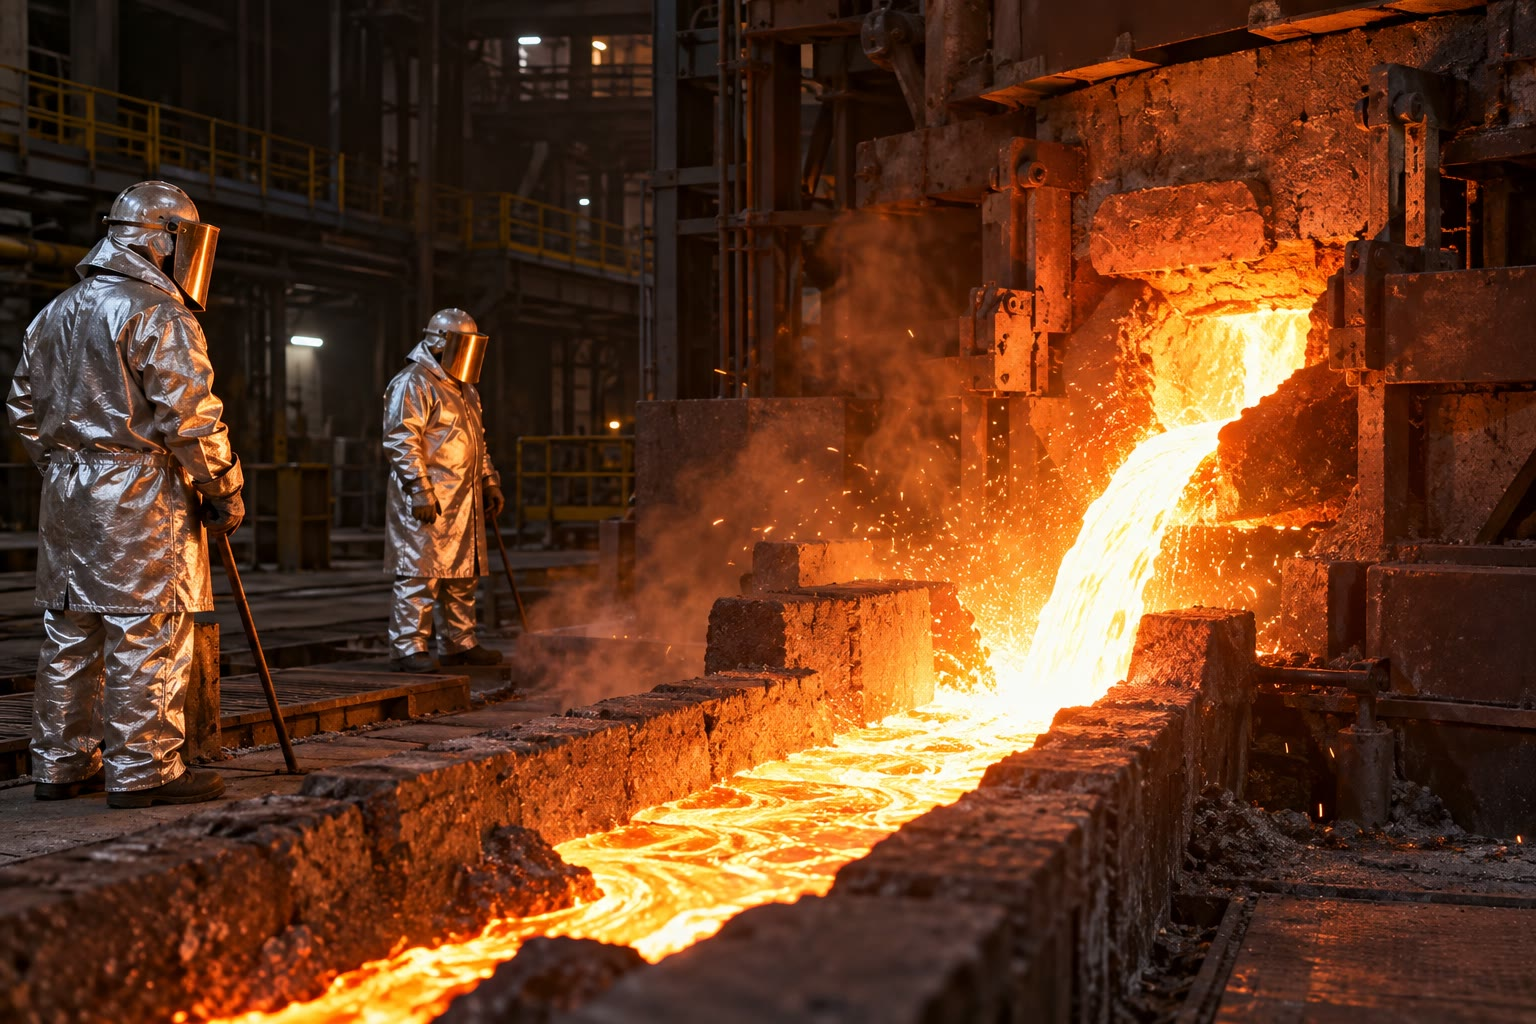
\includegraphics[width=0.62\linewidth]{images/book3/ai/b2-06-blast-furnace.jpg}

{\small Penyadapan tanur tinggi: besi cair mengalir di sepanjang saluran
tahan api, diawasi oleh para pekerja berpakaian pemantul panas. Suhu dan
gas di dalam tanur adalah yang memungkinkan karbon monoksida mengambil
oksigen dari besi oksida.}
\end{omfigure}

\section{Diagram Ellingham}

Untuk membandingkan afinitas berbagai logam terhadap oksigen, reaksi-reaksi
dituliskan sedemikian rupa sehingga semuanya mengonsumsi jumlah yang sama
dari pereaksi bersama itu.

\begin{definition}[Diagram Ellingham]\label{def:b2:ellingham:diagram}
Yang disebut \emph{diagram Ellingham}\index{diagram Ellingham} sekelompok
oksida adalah grafik, terhadap suhu, \omterm{def:b2:reaction-free-energy:gibbs-energy}{energi Gibbs} standar reaksi
pembentukannya yang dituliskan untuk satu mol dioksigen,
\[
  \tfrac{2x}{y}\,\mathrm M + \ce{O2} \longrightarrow \tfrac{2}{y}\,\mathrm{M}_x\mathrm O_y ,
  \qquad \Delta_r G^\circ(T) \ \text{per mol } \ce{O2} .
\]
\end{definition}

Sebagai contoh, \ce{2Zn + O2 -> 2ZnO}, \ce{4/3Al + O2 -> 2/3Al2O3},
\ce{2C + O2 ->
2CO}. Ordinatnya dalam \unit{kJ} per mol \ce{O2}, selalu
negatif untuk logam-logam pada diagram ini.

\begin{proposition}[Garis lurus]\label{prop:b2:ellingham:line}
Dalam \omterm{def:b2:reaction-free-energy:ellingham-approximation}{pendekatan Ellingham}, setiap garis lurus, dengan kemiringan
$-\Delta_r
S^\circ$. Untuk sebuah logam dan oksidanya, yang keduanya
terkondensasi, $\Delta_r S^\circ$ mendekati minus entropi satu mol
dioksigen yang dikonsumsi, sekitar $-\qty{200}{J/(K.mol)}$: garis-garis
itu naik seiring suhu, semuanya dengan kemiringan yang hampir sama.
\end{proposition}

\begin{proof}
$\Delta_r G^\circ = \Delta_r H^\circ - T\Delta_r S^\circ$ dengan $\Delta_r
H^\circ$, $\Delta_r S^\circ$ tetap. Entropi molar padatan berkisar puluhan
\unit{J/(K.mol)} dan sebagian besar saling meniadakan antara logam dan
oksida, sedangkan satu mol gas dikonsumsi, dengan entropi
$S^\circ(\ce{O2}) = \qty{205}{J/(K.mol)}$. Untuk seng,
$2(43.65) - 2(41.63) - 205.15 = \qty{-201.1}{J/(K.mol)}$.
% ledger: s0:ZnO_cr, s0:Zn_cr, s0:O2_g
\end{proof}

\begin{proposition}[Patahan pada garis]\label{prop:b2:ellingham:break}
Pada suhu ketika logam melebur atau mendidih, kemiringan garis berubah:
kemiringannya bertambah sebesar $\nu\,\Delta_{\text{trs}}S$, dengan $\nu$
jumlah logam dalam reaksi dan
$\Delta_{\text{trs}}S = \Delta_{\text{trs}}H/T_{\text{trs}}$. Perubahan
wujud oksida justru mengurangi kemiringannya.
\end{proposition}

\begin{proof}
Di atas suhu transisi, logam bereaksi dari fasenya yang baru, yang
entropinya lebih tinggi sebesar $\Delta_{\text{trs}}S$: $\Delta_r S^\circ$
berkurang sebesar $\nu\,\Delta_{\text{trs}}S$ dan kemiringan
$-\Delta_r S^\circ$ bertambah sebesar itu pula. $\Delta_r G^\circ$
sendiri kontinu, karena pada $T_{\text{trs}}$ kedua fase mempunyai
\omterm{def:b2:chemical-potential:chemical-potential}{potensial kimia} yang sama. Untuk oksida, tandanya berlawanan.
\end{proof}

Peleburan mengubah kemiringan sedikit; pendidihan, yang mengubah pereaksi
terkondensasi menjadi gas, mengubahnya banyak. Seng mendidih pada
\qty{1180}{K}: di atas suhu itu, pembentukan seng oksida mengonsumsi tiga
mol gas per dua mol oksida, dan garisnya menanjak tajam. Hal yang sama
terjadi pada magnesium di atas titik didihnya.

\begin{omfigure}
\begin{tikzpicture}[lab/.style={anchor=west, font=\scriptsize, inner sep=1pt}]
\begin{axis}[omellingham,
  width=0.84\linewidth, height=11cm, xmin=300, xmax=2100, ymin=-1250, ymax=0,
  clip mode=individual,
  xlabel={$T$ (K)}, ylabel={$\Delta_r G^\circ$ (\unit{kJ} per mol \ce{O2})},
  xtick={300,500,700,900,1100,1300,1500,1700,1900,2100},
  x tick label style={rotate=45, anchor=north east, font=\scriptsize}]
\addplot[black!60, thick] table[x=T, y=G] {figdata/out/bachelor-2-ellingham-a-HgO.dat};
\addplot[omProp, thick] table[x=T, y=G] {figdata/out/bachelor-2-ellingham-a-Cu2O.dat};
\addplot[omDef, thick] table[x=T, y=G] {figdata/out/bachelor-2-ellingham-a-FeO.dat};
\addplot[omExo, very thick] table[x=T, y=G] {figdata/out/bachelor-2-ellingham-a-ZnO.dat};
\addplot[black!60, thick] table[x=T, y=G] {figdata/out/bachelor-2-ellingham-a-Cr2O3.dat};
\addplot[omProp, thick] table[x=T, y=G] {figdata/out/bachelor-2-ellingham-a-TiO2.dat};
\addplot[omDef, thick] table[x=T, y=G] {figdata/out/bachelor-2-ellingham-a-Al2O3.dat};
\addplot[black!60, thick] table[x=T, y=G] {figdata/out/bachelor-2-ellingham-a-MgO.dat};
\addplot[omProp, thick] table[x=T, y=G] {figdata/out/bachelor-2-ellingham-a-CaO.dat};
\addplot[omThm, very thick] table[x=T, y=G] {figdata/out/bachelor-2-ellingham-a-C-CO.dat};
\addplot[omThm, thick, dashed] table[x=T, y=G] {figdata/out/bachelor-2-ellingham-a-C-CO2.dat};
\addplot[omThm, thick, dotted] table[x=T, y=G] {figdata/out/bachelor-2-ellingham-a-CO-CO2.dat};
\addplot[omDef, thick, dashed] table[x=T, y=G] {figdata/out/bachelor-2-ellingham-a-H2-H2O.dat};
% labels: inside for the two short lines, at the right end for the others
\node[font=\scriptsize, black!70, anchor=south] at (axis cs:400,-60) {\ce{HgO}};
\node[font=\scriptsize, omProp, anchor=south] at (axis cs:1100,-150) {\ce{Cu2O}};
\draw[omExo, thin] (axis cs:2100,-69) -- (axis cs:2150,-60) node[lab, text=omExo] {\ce{ZnO}};
\draw[omThm, thin] (axis cs:2100,-204) -- (axis cs:2150,-185) node[lab, text=omThm] {\ce{CO}/\ce{CO2}};
\draw[omDef, thin] (axis cs:2100,-259) -- (axis cs:2150,-235) node[lab, text=omDef] {\ce{H2}/\ce{H2O}};
\draw[omDef, thin] (axis cs:2100,-286) -- (axis cs:2150,-285) node[lab, text=omDef] {\ce{FeO}};
\draw[black!70, thin] (axis cs:2100,-393) -- (axis cs:2150,-365) node[lab, text=black!70] {\ce{Cr2O3}};
\draw[omThm, thin] (axis cs:2100,-396) -- (axis cs:2150,-415) node[lab, text=omThm] {\ce{C}/\ce{CO2}};
\draw[omProp, thin] (axis cs:2100,-567) -- (axis cs:2150,-540) node[lab, text=omProp] {\ce{TiO2}};
\draw[omThm, thin] (axis cs:2100,-589) -- (axis cs:2150,-590) node[lab, text=omThm] {\ce{C}/\ce{CO}};
\draw[black!70, thin] (axis cs:2100,-600) -- (axis cs:2150,-640) node[lab, text=black!70] {\ce{MgO}};
\draw[omDef, thin] (axis cs:2100,-668) -- (axis cs:2150,-690) node[lab, text=omDef] {\ce{Al2O3}};
\draw[omProp, thin] (axis cs:2100,-765) -- (axis cs:2150,-765) node[lab, text=omProp] {\ce{CaO}};
\end{axis}
\end{tikzpicture}

{\small \omterm{def:b2:ellingham:diagram}{Diagram Ellingham}: \omterm{def:b2:reaction-free-energy:gibbs-energy}{energi Gibbs} pembentukan standar oksida per mol
\ce{O2}, terhadap suhu, dari \omterm{def:b2:reaction-free-energy:gibbs-energy}{energi Gibbs} yang ditabelkan. Makin rendah
sebuah garis, makin stabil oksidanya dan makin kuat sifat pereduksi
logamnya. Setiap garis logam diberi label dengan oksidanya; \ce{C}/\ce{CO}
adalah \ce{2C + O2 -> 2CO}, \ce{C}/\ce{CO2} adalah \ce{C + O2 -> CO2},
\ce{CO}/\ce{CO2} adalah \ce{2CO + O2 -> 2CO2}, dan \ce{H2}/\ce{H2O}
adalah \ce{2H2 + O2 -> 2H2O}, dengan air berupa gas.}
% ledger: janafG:Cu2O.300, janafG:FeO.300, janafG:Cr2O3.300, janafG:TiO2.500, janafG:Al2O3.300, janafG:MgO.300, janafG:CaO.300, janafG:CO.300, janafG:CO2.300, janafG:H2O.300, dfh:ZnO_cr, dfh:HgO_cr, s0:HgO_cr, s0:Hg_l, s0:Hg_g, dfh:Hg_g (all temperatures in figdata/bachelor-2/ellingham.py)
\end{omfigure}

\section{Membaca diagram}

\begin{definition}[Tekanan oksigen kesetimbangan]\label{def:b2:ellingham:oxygen-pressure}
Yang disebut \emph{tekanan oksigen kesetimbangan}\index{tekanan oksigen kesetimbangan}
sebuah pasangan logam–oksida pada suhu $T$ adalah tekanan dioksigen
tempat logam dan oksida berdampingan dalam kesetimbangan:
$RT\ln(p_{\ce{O2}}/p^\circ) = \Delta_r
G^\circ(T)$ untuk reaksi yang
dituliskan per mol \ce{O2}.
\end{definition}

\begin{theorem}[Daerah logam dan daerah oksida]\label{thm:b2:ellingham:domains}
Dalam atmosfer bertekanan oksigen $p_{\ce{O2}}$ pada suhu $T$, logam
teroksidasi jika $RT\ln(p_{\ce{O2}}/p^\circ) > \Delta_r G^\circ(T)$, dan
oksida tereduksi menjadi logam jika $RT\ln(p_{\ce{O2}}/p^\circ) < \Delta_r
G^\circ(T)$. Pada diagram, oksida stabil di atas garisnya, logam di
bawahnya.
\end{theorem}

\begin{proof}
Dengan logam dan oksida terkondensasi beraktivitas 1, $Q = p^\circ/p_{\ce{O2}}$
dan $\Delta_r G = \Delta_r G^\circ + RT\ln Q = \Delta_r G^\circ - RT\ln(p_{\ce{O2}}/
p^\circ)$. Oksidasi berjalan ke arah maju jika $\Delta_r G < 0$.
\end{proof}

Di udara ($p_{\ce{O2}} = \qty{0.21}{bar}$, $RT\ln 0.21$ bernilai
\qty{-4}{kJ/mol} pada suhu kamar dan \qty{-13}{kJ/mol} pada
\qty{1000}{K}, hampir nol pada skala ini), setiap logam pada diagram yang
garisnya berada di bawah sumbu teroksidasi: pada suhu kamar semuanya,
bahkan tembaga. Hanya oksida-oksida di dekat bagian atas (perak, raksa)
yang terurai pada pemanasan sedang.

\begin{example}[Oksida raksa]\label{ex:b2:ellingham:hgo}
Untuk \ce{2Hg + O2 -> 2HgO}, nilai-nilai kunci CODATA memberikan
$\Delta_r H^\circ =
\qty{-181.6}{kJ/mol}$ dengan raksa cair; di atas titik
didih raksa, logamnya berupa gas dan $\Delta_r H^\circ = \qty{-304.3}{kJ/mol}$, $\Delta_r
S^\circ = \qty{-414.6}{J/(K.mol)}$. Garis
itu memotong nol pada $T = 304.3/0.4146 \approx \qty{734}{K}$: jika
dipanaskan di atas suhu itu di udara, atau di bawah \qty{1}{bar} oksigen,
raksa oksida merah melepaskan oksigennya --- cara oksigen pertama kali
diisolasi pada tahun 1774.
% ledger: dfh:HgO_cr, s0:HgO_cr, s0:Hg_l, s0:Hg_g, dfh:Hg_g, s0:O2_g (computed in figdata/bachelor-2/ellingham.py)
\end{example}

\begin{proposition}[Logam mana mereduksi oksida mana]\label{prop:b2:ellingham:reduction}
Pada suhu tertentu, logam M mereduksi oksida logam N, pada kondisi
standar, jika garis M terletak di bawah garis N. \omterm{def:b2:reaction-free-energy:reaction-gibbs}{Energi Gibbs reaksi
standar} reduksi itu, per mol \ce{O2} yang dipindahkan, adalah selisih
kedua ordinat.
\end{proposition}

\begin{proof}
Reduksi itu adalah pembentukan oksida M dikurangi pembentukan oksida N,
keduanya per mol \ce{O2}: $\Delta_r G^\circ = \Delta_r G^\circ_{\mathrm M} - \Delta_r
G^\circ_{\mathrm N}$, negatif jika garis M lebih rendah.
\end{proof}

\begin{method}[Membaca diagram Ellingham]\label{met:b2:ellingham:read-ellingham}
\begin{enumerate}
  \item Carilah kedua garis pada suhu yang dikehendaki. Garis yang lebih
        rendah adalah oksida yang lebih stabil; logamnya mereduksi oksida
        yang lain.
  \item Jarak vertikalnya adalah $\Delta_r G^\circ$ per mol \ce{O2}: jarak
        \qty{100}{kJ} atau lebih berarti reduksi yang praktis tuntas.
  \item Di tempat dua garis berpotongan, arah reduksi berbalik: bacalah
        suhu perpotongannya.
  \item Perhatikan patahan-patahannya: logam yang mendidih di dalam selang
        itu keluar sebagai uap, yang dapat dipisahkan dengan distilasi ---
        atau yang teroksidasi kembali ketika didinginkan.
\end{enumerate}
\end{method}

\begin{definition}[Reduksi aluminotermik]\label{def:b2:ellingham:aluminothermy}
Yang disebut \emph{reduksi aluminotermik}\index{reduksi aluminotermik}
adalah reduksi oksida logam oleh serbuk aluminium, yang mungkin untuk
setiap oksida yang garisnya terletak di atas garis alumina, dan begitu
\omterm{def:b2:reaction-enthalpy:exothermic}{eksoterm} sehingga campurannya meleleh: \ce{Fe2O3 + 2Al -> Al2O3 + 2Fe}
(termit) mengelas rel; \ce{Cr2O3 + 2Al ->
Al2O3 + 2Cr} menghasilkan kromium
yang bebas karbon.
\end{definition}

\begin{omfigure}
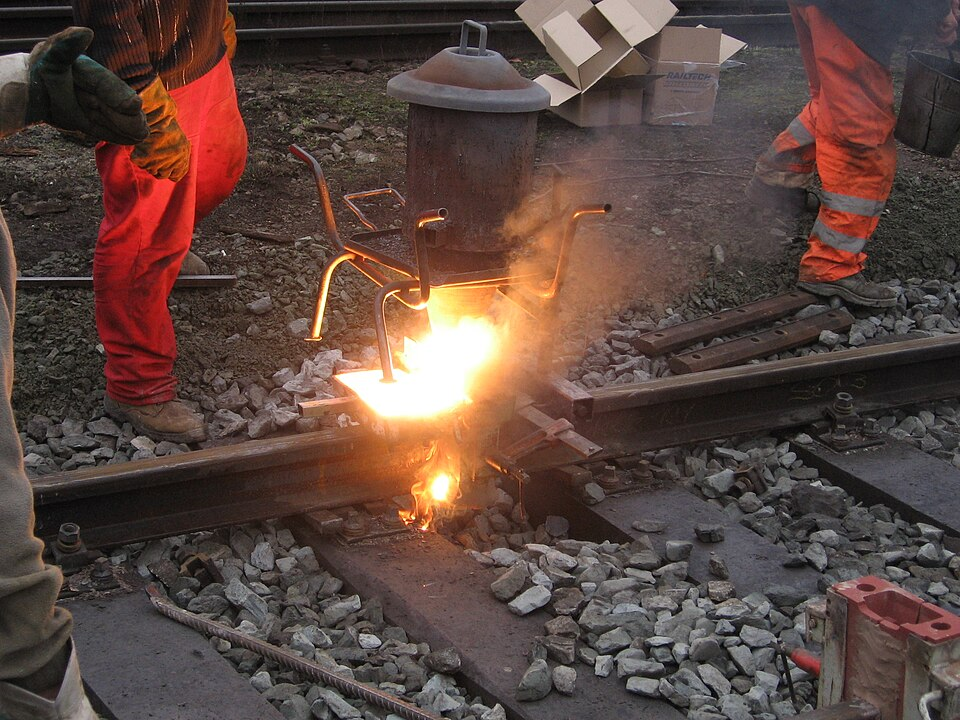
\includegraphics[width=0.5\linewidth]{images/book3/thermite.jpg}

{\small Pengelasan termit pada rel: reaksi besi oksida dengan aluminium di
dalam krusibel di atas sambungan menghasilkan besi cair, yang mengalir ke
bawah ke dalam cetakan di antara kedua ujung rel. (Foto: PetrS., CC BY-SA
3.0, Wikimedia Commons.)}
\end{omfigure}

\section{Karbon dan karbon monoksida}

Tiga garis melibatkan karbon:
\begin{itemize}
  \item \ce{C + O2 -> CO2}: satu mol gas menghasilkan satu mol gas,
        $\Delta_r S^\circ
        \approx 0$, garis yang hampir mendatar di dekat
        \qty{-395}{kJ};
  \item \ce{2C + O2 -> 2CO}: satu mol gas menghasilkan dua mol gas,
        $\Delta_r S^\circ
        \approx \qty{+180}{J/(K.mol)}$, garis yang
        \emph{turun} seiring suhu;
  \item \ce{2CO + O2 -> 2CO2}: tiga mol gas menghasilkan dua mol gas, garis
        yang naik.
\end{itemize}

\begin{proposition}[Karbon mereduksi hampir semuanya pada suhu tinggi]\label{prop:b2:ellingham:carbon}
Garis \ce{2C + O2 -> 2CO} turun seiring suhu dan memotong garis sebagian
besar oksida logam: di atas suhu perpotongan, karbon mereduksi oksida itu,
dengan menghasilkan karbon monoksida. Perpotongan untuk besi(II) oksida
berada di dekat \qty{1040}{K}, untuk seng oksida di dekat \qty{1220}{K};
untuk titania dan magnesia perpotongannya berada di dekat atau di atas
\qty{2000}{K}, untuk alumina lebih tinggi lagi, tempat logam-logam itu
bergabung dengan karbon menjadi karbida atau teroksidasi kembali ketika
gasnya mendingin.
\end{proposition}

\begin{proof}
Kemiringan $-\Delta_r S^\circ$ garis karbon negatif
($\Delta\nu_{\text{gas}}
= +1$), sedangkan kemiringan garis-garis oksida
positif: keduanya berpotongan sekali. Suhu-suhunya dibaca pada garis-garis
yang dihitung.
% ledger: janafG:CO.900, janafG:CO.1100, janafG:FeO.900, janafG:FeO.1100 (crossings computed in figdata/bachelor-2/ellingham.py)
\end{proof}

\begin{definition}[Kesetimbangan Boudouard]\label{def:b2:ellingham:boudouard}
Yang disebut \emph{kesetimbangan Boudouard}\index{kesetimbangan Boudouard}
adalah \ce{C(s) + CO2(g) <=> 2CO(g)}, yang \omterm{def:b2:reaction-enthalpy:exothermic}{endoterm}, antara karbon dan
kedua oksida karbon.
\end{definition}

\begin{proposition}[Komposisi gas di atas karbon]\label{prop:b2:ellingham:boudouard}
Sistem karbon + \ce{CO} + \ce{CO2} mempunyai \omterm{def:b2:equilibrium-shifts:variance}{varians} 2: pada $T$ dan
tekanan total $p$ tertentu, fraksi mol $x$ karbon monoksida ditetapkan oleh
$x^2/(1 - x)
= K^\circ(T)\,p^\circ/p$. Pada \qty{1}{bar}, gasnya hampir
murni \ce{CO2} di bawah \qty{700}{K} dan hampir murni \ce{CO} di atas
\qty{1200}{K}; perpotongan ketiga garis karbon, di dekat \qty{975}{K},
adalah tempat $K^\circ = 1$.
\end{proposition}

\begin{proof}
Tiga spesies, satu reaksi, dua fase: $v = 3 - 1 + 2 - 2 = 2$. Dengan
$p_{\ce{CO}}
= xp$ dan $p_{\ce{CO2}} = (1 - x)p$,
$Q = x^2p/[(1 - x)p^\circ]$. Pada $K^\circ = 1$, \omterm{def:b2:reaction-free-energy:gibbs-energy}{energi Gibbs} standar
\ce{2C + O2 -> 2CO} dan \ce{C + O2 -> CO2} sama: kedua garis itu, dan
dengan demikian garis ketiga, bertemu.
\end{proof}

\begin{omfigure}
\begin{tikzpicture}
\begin{axis}[
  width=0.62\linewidth, height=5.4cm, xmin=500, xmax=1500, ymin=0, ymax=1.05,
  axis x line=bottom, axis y line=left, xlabel={$T$ (K)},
  xtick={500,700,900,1100,1300,1500}, ytick={0,0.5,1},
  ylabel={fraksi mol \ce{CO}}, tick label style={font=\small},
  label style={font=\small}, clip=false]
\addplot[omThm, very thick] table[x=T, y=xCO] {figdata/out/bachelor-2-ellingham-b.dat};
\node[font=\scriptsize, anchor=west] at (axis cs:1150,0.55) {\ce{CO} stabil};
\node[font=\scriptsize, anchor=west] at (axis cs:510,0.6) {\ce{CO2} (dan karbon) stabil};
\end{axis}
\end{tikzpicture}

{\small \omterm{def:b2:ellingham:boudouard}{Kesetimbangan Boudouard} pada \qty{1}{bar}: fraksi mol karbon
monoksida dalam gas yang berada dalam kesetimbangan dengan karbon.}
% ledger: janafG:CO.700, janafG:CO2.700, janafG:CO.1100, janafG:CO2.1100 (computed in figdata/bachelor-2/ellingham.py)
\end{omfigure}

\section{Tanur tinggi}

Bijih besi (hematit \ce{Fe2O3}, magnetit \ce{Fe3O4}), kokas, dan batu
kapur dimasukkan di puncak sebuah cerobong yang tinggi; udara panas
ditiupkan di dekat dasar. Sambil turun, padatan bertemu dengan gas panas
yang naik; gas itu keluar di puncak dalam keadaan sudah dingin.
\begin{itemize}
  \item Di tuyer, kokas terbakar dalam udara panas: \ce{C + O2 -> CO2}, dan
        di atasnya, dengan karbon berlebih, \ce{CO2 + C -> 2CO}
        (Boudouard): gas yang naik sebagian besar berupa karbon monoksida
        dan nitrogen.
  \item Di bagian atas, karbon monoksida mereduksi besi oksida tahap demi
        tahap, \ce{3Fe2O3 + CO -> 2Fe3O4 + CO2}, \ce{Fe3O4 + CO -> 3FeO + CO2},
        \ce{FeO + CO -> Fe + CO2}. Dua tahap pertama mudah; untuk tahap
        terakhir, garis \ce{CO}/\ce{CO2} berada sedikit \textit{di atas}
        garis \ce{FeO}: \omterm{def:b2:reaction-free-energy:reaction-gibbs}{energi Gibbs reaksi standarnya} sedikit positif
        ($K^\circ \approx 0.3$ pada \qty{900}{K}), dan reduksinya
        memerlukan gas yang mengandung \ce{CO} paling sedikit tiga kali
        lebih banyak daripada \ce{CO2} --- yang disediakan oleh
        \omterm{def:b2:ellingham:boudouard}{kesetimbangan Boudouard} di zona panas di bawahnya.
  \item Di bagian yang lebih bawah dan lebih panas, karbon sendiri
        mereduksi sisanya, \ce{FeO + C ->
        Fe + CO}; besi melarutkan karbon,
        meleleh, dan terkumpul di dasar bersama terak cair yang dibentuk
        oleh kapur dan silika dari bijih.
\end{itemize}

\begin{omfigure}
\begin{tikzpicture}[font=\small, >={Stealth}]
  \fill[gray!12] (-1.4,0) -- (-2.0,3.0) -- (-1.3,7.0) -- (1.3,7.0) -- (2.0,3.0) -- (1.4,0) -- cycle;
  \draw[thick] (-1.4,0) -- (-2.0,3.0) -- (-1.3,7.0) (1.4,0) -- (2.0,3.0) -- (1.3,7.0);
  \draw[thick] (-1.4,0) -- (1.4,0);
  \fill[orange!70!red] (-1.4,0) rectangle (1.4,0.35);
  \fill[yellow!50!orange] (-1.45,0.35) rectangle (1.45,0.6);
  \node[font=\scriptsize] at (0,0.17) {besi cair};
  \node[font=\scriptsize] at (0,0.48) {terak};
  % tuyeres
  \draw[->, thick, omDef] (-3.2,1.2) -- (-1.75,1.2) node[pos=0, left] {udara panas};
  \draw[->, thick, omDef] (3.2,1.2) -- (1.75,1.2);
  % charge and gas
  \draw[->, thick] (-0.6,7.9) -- (-0.6,7.1) node[pos=0, above left, xshift=6pt] {bijih, kokas, batu kapur};
  \draw[->, thick, omThm] (0.7,7.1) -- (0.7,7.9) node[pos=1, above right, xshift=-6pt] {gas puncak (\ce{CO}, \ce{CO2}, \ce{N2})};
  \draw[->, omThm, thick] (0.6,1.6) -- (0.6,6.4);
  \draw[->, thick] (-0.6,6.4) -- (-0.6,1.6);
  \node[omThm, font=\scriptsize, rotate=90] at (0.9,4.0) {gas naik};
  \node[font=\scriptsize, rotate=90] at (-0.9,4.0) {padatan turun};
  % zones
  \node[anchor=west, align=left, font=\scriptsize] at (2.3,6.0) {\ce{3Fe2O3 + CO -> 2Fe3O4 + CO2}\\ \ce{Fe3O4 + CO -> 3FeO + CO2}};
  \node[anchor=west, align=left, font=\scriptsize] at (2.3,4.2) {\ce{FeO + CO -> Fe + CO2}};
  \node[anchor=west, align=left, font=\scriptsize] at (2.3,2.7) {\ce{CO2 + C -> 2CO}\\ \ce{FeO + C -> Fe + CO}};
  \node[anchor=west, align=left, font=\scriptsize] at (2.3,1.6) {\ce{C + O2 -> CO2}};
  \draw[densely dotted] (1.95,6.0) -- (2.3,6.0) (1.9,4.2) -- (2.3,4.2) (2.0,2.8) -- (2.3,2.8);
  \node[anchor=east, align=right, font=\scriptsize, black!60] at (-2.2,6.0) {lebih dingin};
  \node[anchor=east, align=right, font=\scriptsize, black!60] at (-2.2,2.3) {lebih panas};
  \draw[->, black!50] (-2.6,5.6) -- (-2.6,2.7);
\end{tikzpicture}

{\small Tanur tinggi sebagai reaktor arus berlawanan. Padatan turun, gas
pereduksi yang panas naik; besi oksida direduksi oleh karbon monoksida di
bagian atas yang lebih dingin, dan oleh karbon di bagian bawah yang lebih
panas. Besi dan terak disadap di dasar.}
\end{omfigure}

\begin{omfigure}
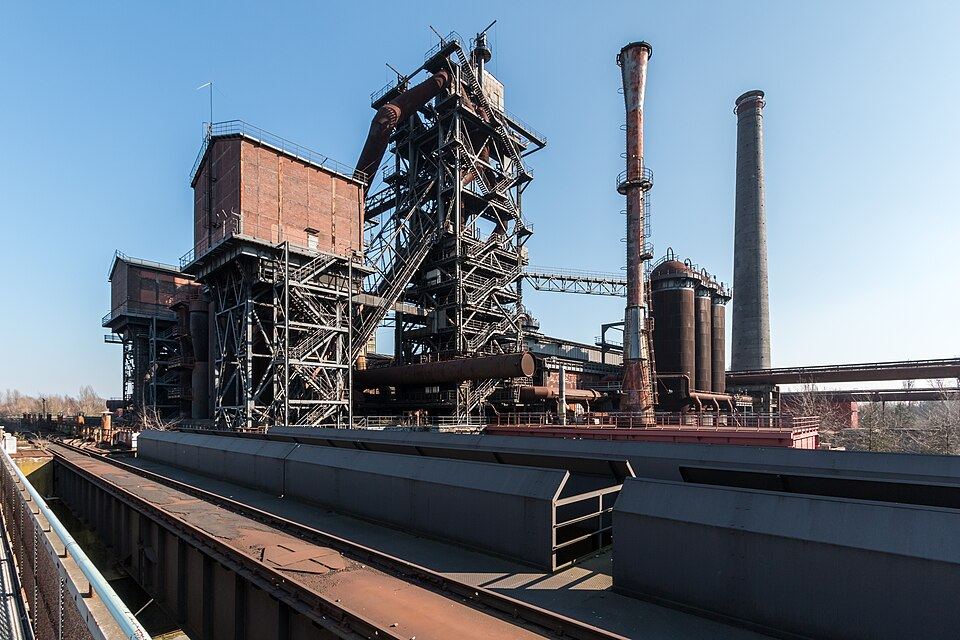
\includegraphics[width=0.6\linewidth]{images/book3/blast-furnace.jpg}

{\small Sebuah tanur tinggi yang dilestarikan sebagai monumen
(Duisburg-Nord, berhenti beroperasi pada tahun 1985): cerobongnya yang
tinggi dengan cincin pipa untuk udara panas, dan saluran gas di
puncaknya. (Foto: Dietmar Rabich, CC BY-SA 4.0, Wikimedia Commons.)}
\end{omfigure}

\section{Jalur lain menuju logam}

\begin{definition}[Pirometalurgi dan hidrometalurgi]\label{def:b2:ellingham:metallurgy}
Yang disebut \emph{pirometalurgi}\index{pirometalurgi} adalah ekstraksi
logam pada suhu tinggi, dengan mereduksi oksidanya di dalam tanur.
Selanjutnya, \emph{hidrometalurgi}\index{hidrometalurgi} mengekstraksinya
dari larutan berair. Tahap-tahap lazimnya adalah
\emph{pemanggangan}\index{pemanggangan} (pemanasan bijih sulfida di udara
untuk mengubahnya menjadi oksida, \ce{2ZnS + 3O2 -> 2ZnO + 2SO2}),
\emph{pelindian}\index{pelindian} (pelarutan senyawa logam itu, sering
dalam asam sulfat, \ce{ZnO + 2H+ ->
Zn^2+ + H2O}), pemurnian larutan,
misalnya dengan \emph{sementasi}\index{sementasi} (reduksi ion-ion logam
yang lebih mulia oleh serbuk logam yang kurang mulia,
\ce{Cu^2+ + Zn -> Cu + Zn^2+}), dan perolehan kembali logamnya, sering
dengan elektrolisis.
\end{definition}

Diagram ini menjelaskan pembagian kerjanya. Besi, seng, timbal, dan timah
diperoleh dengan karbon di dalam tanur. Aluminium, yang garisnya terletak
jauh di bawah garis karbon pada setiap suhu yang dapat dipraktikkan,
dibuat dengan elektrolisis oksidanya yang meleleh
(\cref{ch:b2:batteries-electrolysis}); magnesium dengan elektrolisis atau
dengan reduksi oleh silikon dalam vakum, yang menyingkirkan uap
magnesium; titanium dengan mengubah oksidanya menjadi klorida,
\ce{TiO2 + 2Cl2 + C -> TiCl4 +
CO2} (\cref{exo:b2:reaction-free-energy:12}),
lalu mereduksi kloridanya dengan magnesium (proses Kroll). Sebagian besar
seng dunia dibuat dengan \omterm{def:b2:ellingham:metallurgy}{pemanggangan}, \omterm{def:b2:ellingham:metallurgy}{pelindian}, dan elektrolisis: jalur
\omterm{def:b2:ellingham:metallurgy}{hidrometalurgi} memberikan logam yang lebih murni dan menghindari
penanganan uap seng.

\begin{omfigure}
\begin{tikzpicture}[font=\small, >={Stealth}, box/.style={draw, thick, rounded corners=2pt, align=center, minimum height=0.9cm, fill=white, text width=2.3cm}]
  \node[box] (r) at (0,0) {pemanggangan\\ \ce{ZnS} $\to$ \ce{ZnO}};
  \node[box] (l) at (3.2,0) {pelindian\\ dalam \ce{H2SO4}};
  \node[box] (c) at (6.4,0) {pemurnian\\ (sementasi)};
  \node[box] (e) at (9.6,0) {elektrolisis\\ \ce{Zn^2+} $\to$ \ce{Zn}};
  \draw[->, thick] (r) -- (l); \draw[->, thick] (l) -- (c); \draw[->, thick] (c) -- (e);
  \draw[->, thick, black!60] (r.north) -- ++(0,0.7) node[above] {\ce{SO2} $\to$ asam sulfat};
  \draw[->, thick, omThm] (e.south) -- ++(0,-0.6) -| (l.south) node[pos=0.25, below] {asam dikembalikan};
  \draw[->, thick] (e.east) -- ++(0.8,0) node[right] {seng};
\end{tikzpicture}

{\small Jalur \omterm{def:b2:ellingham:metallurgy}{hidrometalurgi} menuju seng. Belerang dioksida dari
\omterm{def:b2:ellingham:metallurgy}{pemanggangan} dijadikan asam sulfat untuk \omterm{def:b2:ellingham:metallurgy}{pelindian}; asam yang diregenerasi
di anode elektrolisis dikembalikan ke \omterm{def:b2:ellingham:metallurgy}{pelindian}.}
\end{omfigure}

\section{Latihan}

\begin{exercise}[$\star$]\label{exo:b2:ellingham:1}
Tuliskan reaksi-reaksi yang diwakili oleh garis tembaga(I) oksida,
alumina, karbon monoksida, dan karbon dioksida, masing-masing untuk satu
mol \ce{O2}.
\end{exercise}

\begin{exercise}[$\star$]\label{exo:b2:ellingham:2}
Dari nilai-nilai kunci CODATA ($\Delta_f H^\circ(\ce{ZnO}) = \qty{-350.46}{kJ/mol}$,
$S^\circ$: \ce{ZnO} 43.65, \ce{Zn} 41.63, \ce{O2} \qty{205.15}{J/(K.mol)}),
tuliskan $\Delta_r G^\circ(T)$ untuk \ce{2Zn + O2 -> 2ZnO} dengan seng
padat.
\end{exercise}

\begin{exercise}[$\star$]\label{exo:b2:ellingham:3}
Dengan diagram itu, daftarlah logam-logam yang dapat mereduksi
kromium(III) oksida pada \qty{1500}{K}, dan logam-logam yang tidak dapat.
\end{exercise}

\begin{exercise}[$\star$]\label{exo:b2:ellingham:4}
Jelaskan tanda kemiringan setiap garis dari ketiga garis karbon.
\end{exercise}

\begin{exercise}[$\star\star$]\label{exo:b2:ellingham:5}
Hitunglah \omterm{def:b2:ellingham:oxygen-pressure}{tekanan oksigen kesetimbangan} raksa(II) oksida pada
\qty{600}{K} (raksa cair, $\Delta_r H^\circ = \qty{-181.6}{kJ}$,
$\Delta_r S^\circ =
\qty{-216.5}{J/K}$ per mol \ce{O2}). Apakah raksa
teroksidasi di udara pada suhu itu?
\end{exercise}

\begin{exercise}[$\star\star$]\label{exo:b2:ellingham:6}
Hitunglah $\Delta_r G^\circ$ pada \qty{298}{K} untuk reaksi termit,
\ce{Fe2O3 +
2Al -> Al2O3 + 2Fe}, jika diketahui $\Delta_f G^\circ = \qty{-743.5}{kJ/mol}$ untuk \ce{Fe2O3} dan \qty{-1582.3}{kJ/mol} untuk
\ce{Al2O3}, lalu jelaskan mengapa reaksi itu, walaupun sangat \omterm{def:b2:reaction-free-energy:exergonic}{eksergonik},
tidak mulai berjalan pada suhu kamar.
% ledger: janafG:Fe2O3.298, janafG:Al2O3.298
\end{exercise}

\begin{exercise}[$\star\star$]\label{exo:b2:ellingham:7}
Carilah pada diagram suhu yang di atasnya karbon mereduksi besi(II)
oksida menjadi besi dengan membentuk karbon monoksida, lalu tuliskan
reaksinya.
\end{exercise}

\begin{exercise}[$\star\star$]\label{exo:b2:ellingham:8}
Pada \qty{1100}{K}, $\Delta_f G^\circ(\ce{CO}) = \qty{-209.1}{kJ/mol}$ dan
$\Delta_f G^\circ(\ce{CO2}) = \qty{-396.0}{kJ/mol}$. Hitunglah $K^\circ$
\omterm{def:b2:ellingham:boudouard}{kesetimbangan Boudouard} dan fraksi mol karbon monoksida di atas karbon pada
\qty{1}{bar}. Apa yang terjadi pada gas itu, jika bersentuhan dengan jelaga
atau besi, ketika didinginkan sampai \qty{700}{K}?
% ledger: janafG:CO.1100, janafG:CO2.1100
\end{exercise}

\begin{exercise}[$\star\star$]\label{exo:b2:ellingham:9}
Hidrogen kadang-kadang dipakai untuk mereduksi wolfram oksida. Dengan
garis air, jelaskan mengapa hidrogen merupakan reduktor yang lebih baik
daripada karbon monoksida pada suhu tinggi, tetapi lebih buruk pada suhu
rendah.
\end{exercise}

\begin{exercise}[$\star\star\star$]\label{exo:b2:ellingham:10}
Magnesium oksida dapat direduksi oleh silikon, \ce{2MgO + Si -> SiO2 + 2Mg},
walaupun garis silika terletak di atas garis magnesia pada setiap suhu
dalam diagram. Pada \qty{1500}{K}, magnesium berupa gas dan tabel
memberikan, per mol \ce{O2}, \qty{-845.5}{kJ} untuk magnesia dan
\qty{-643.7}{kJ} untuk silika. Hitunglah $\Delta_r G^\circ$ reduksi itu,
lalu tekanan uap magnesium yang di bawahnya reduksi berjalan ke arah maju.
Bagaimana tanur vakum memanfaatkan hal ini?
% ledger: janafG:MgO.1500, janafG:SiO2.1500
\end{exercise}

\begin{exercise}[$\star\star\star$]\label{exo:b2:ellingham:11}
Hitunglah \omterm{def:b2:equilibrium-shifts:variance}{varians} sistem \ce{FeO(s)}, \ce{Fe(s)}, \ce{CO(g)}, \ce{CO2(g)}
dalam kesetimbangan. Apa artinya bagi gas yang keluar dari bagian atas
tanur tinggi?
\end{exercise}

\begin{exercise}[$\star\star\star$]\label{exo:b2:ellingham:12}
Tembaga dimurnikan dari larutan \omterm{def:b2:ellingham:metallurgy}{pelindiannya} dengan \omterm{def:b2:ellingham:metallurgy}{sementasi} memakai
skrap besi. Dengan potensial standar dari jilid Tahun 1
($E^\circ(\ce{Cu^2+}/\ce{Cu})
= \qty{0.34}{V}$,
$E^\circ(\ce{Fe^2+}/\ce{Fe}) = \qty{-0.41}{V}$), hitunglah tetapan
kesetimbangan \ce{Cu^2+ + Fe -> Cu + Fe^2+} dan konsentrasi sisa ion
tembaga jika larutan itu mengandung \qty{1.0}{mol/L} \ce{Fe^2+}.
\end{exercise}

\section{Soal: Seng dari Api}

\begin{problem}[{Soal akhir pekan --- garis Ellingham seng oksida dan
karbon monoksida, suhu ketika karbon mereduksi seng oksida, varians tanur,
dan pengembunan uap seng}]
\label{pb:b2:ellingham:1}
Sebelum ada elektrolisis, seng dibuat dengan memanaskan oksidanya bersama
karbon di dalam retort tanah liat. Data (CODATA, dan tabel JANAF untuk
seng): $\Delta_f H^\circ(\ce{ZnO})
= \qty{-350.46}{kJ/mol}$; $S^\circ$
(\unit{J/(K.mol)}): \ce{ZnO} 43.65, \ce{Zn} 41.63, \ce{O2} 205.15; seng
melebur pada \qty{692.7}{K} ($\Delta_{\text{fus}}H =
\qty{7.32}{kJ/mol}$)
dan mendidih pada \qty{1180.2}{K} di bawah \qty{1}{bar}
($\Delta_{\text{vap}}H = \qty{115.3}{kJ/mol}$). Untuk \ce{2C + O2 -> 2CO},
tabel memberikan $\Delta_r G^\circ = \qty{-418.2}{kJ}$ pada \qty{1100}{K}
dan \qty{-453.0}{kJ} pada \qty{1300}{K}.
% ledger: dfh:ZnO_cr, s0:ZnO_cr, s0:Zn_cr, s0:O2_g, hT:Zn_cr.692, hT:Zn_l.692, hT:Zn_l.1180, hT:Zn_g.1180, dfh:Zn_g, janafG:CO.1100, janafG:CO.1300

\medskip
\noindent\textbf{Bagian I --- Garis seng oksida.}
\begin{enumerate}
  \item Hitunglah $\Delta_r H^\circ$ dan $\Delta_r S^\circ$ untuk
        \ce{2Zn(s) + O2 ->
        2ZnO} pada \qty{298}{K}.
  \item Tuliskan $\Delta_r G^\circ(T)$ di bawah titik lebur.
  \item Hitunglah entropi peleburan dan entropi penguapan seng.
  \item Tuliskan $\Delta_r G^\circ(T)$ di antara titik lebur dan titik
        didih.
  \item Tuliskan ungkapan itu di atas titik didih.
  \item Hitunglah ketiga kemiringan itu dan jelaskan mengapa yang terakhir
        jauh lebih curam.
  \item Periksalah bahwa ketiga ungkapan itu sesuai pada suhu-suhu
        transisinya.
\end{enumerate}

\medskip
\noindent\textbf{Bagian II --- Garis karbon.}
\begin{enumerate}[resume]
  \item Dari kedua nilai tabel itu, tuliskan garis \ce{2C + O2 -> 2CO}
        dalam bentuk $a + bT$ antara \qty{1100}{K} dan \qty{1300}{K}.
  \item Simpulkan $\Delta_r S^\circ$-nya dan jelaskan tandanya.
  \item Tuliskan reduksi \ce{ZnO + C -> Zn(g) + CO} dan $\Delta_r
        G^\circ(T)$-nya sebagai selisih kedua garis (per mol \ce{O2}).
  \item Tentukan suhu tempat kedua garis itu berpotongan.
  \item Mengapa penting bahwa suhu ini berada di atas titik didih seng?
\end{enumerate}

\medskip
\noindent\textbf{Bagian III --- Retort.}
\begin{enumerate}[resume]
  \item Hitunglah \omterm{def:b2:equilibrium-shifts:variance}{varians} sistem \ce{ZnO(s)}, \ce{C(s)}, \ce{Zn(g)},
        \ce{CO(g)}, dengan seng dan karbon monoksida yang hanya terbentuk
        melalui reduksi.
  \item Dalam retort pada \qty{1300}{K} di bawah \qty{1}{bar}, berapakah
        tekanan parsial seng dan karbon monoksida jika reaksinya tuntas?
  \item Hitunglah $\Delta_r G^\circ$ reduksi itu pada \qty{1300}{K} dan
        $K^\circ$ yang bersesuaian.
  \item Jelaskan mengapa retort dioperasikan sedikit di atas suhu
        perpotongan dan tidak jauh di atasnya.
\end{enumerate}

\medskip
\noindent\textbf{Bagian IV --- Kondensor.}
\begin{enumerate}[resume]
  \item Uap seng dialirkan ke dalam kondensor yang lebih dingin. Tuliskan
        reaksi yang dapat mengoksidasi kembali uap seng oleh karbon
        dioksida.
  \item Dengan diagram itu, jelaskan mengapa gasnya harus dijaga bebas
        dari karbon dioksida.
  \item Mengapa seng harus diembunkan dengan cepat, bukan perlahan-lahan?
  \item Hitunglah massa karbon yang diperlukan per ton seng, dengan
        menganggap reduksinya sesuai dengan yang dituliskan.
  \item Hitunglah kalor yang diserap per ton seng oleh reduksi pada sekitar
        \qty{1300}{K} (ambillah $\Delta_r H^\circ$ dari ungkapan-ungkapan
        pada Bagian I dan II).
  \item Nyatakan suhu yang di atasnya karbon mereduksi seng oksida pada
        kondisi standar.
\end{enumerate}
\end{problem}
